\documentclass[12pt]{article}
\usepackage{parskip, enumerate}
\usepackage{amsmath,pdfpages}
\usepackage{fancyvrb}
\usepackage[vlined,linesnumbered]{algorithm2e}
\usepackage[margin=.6in]{geometry}
\begin{document}
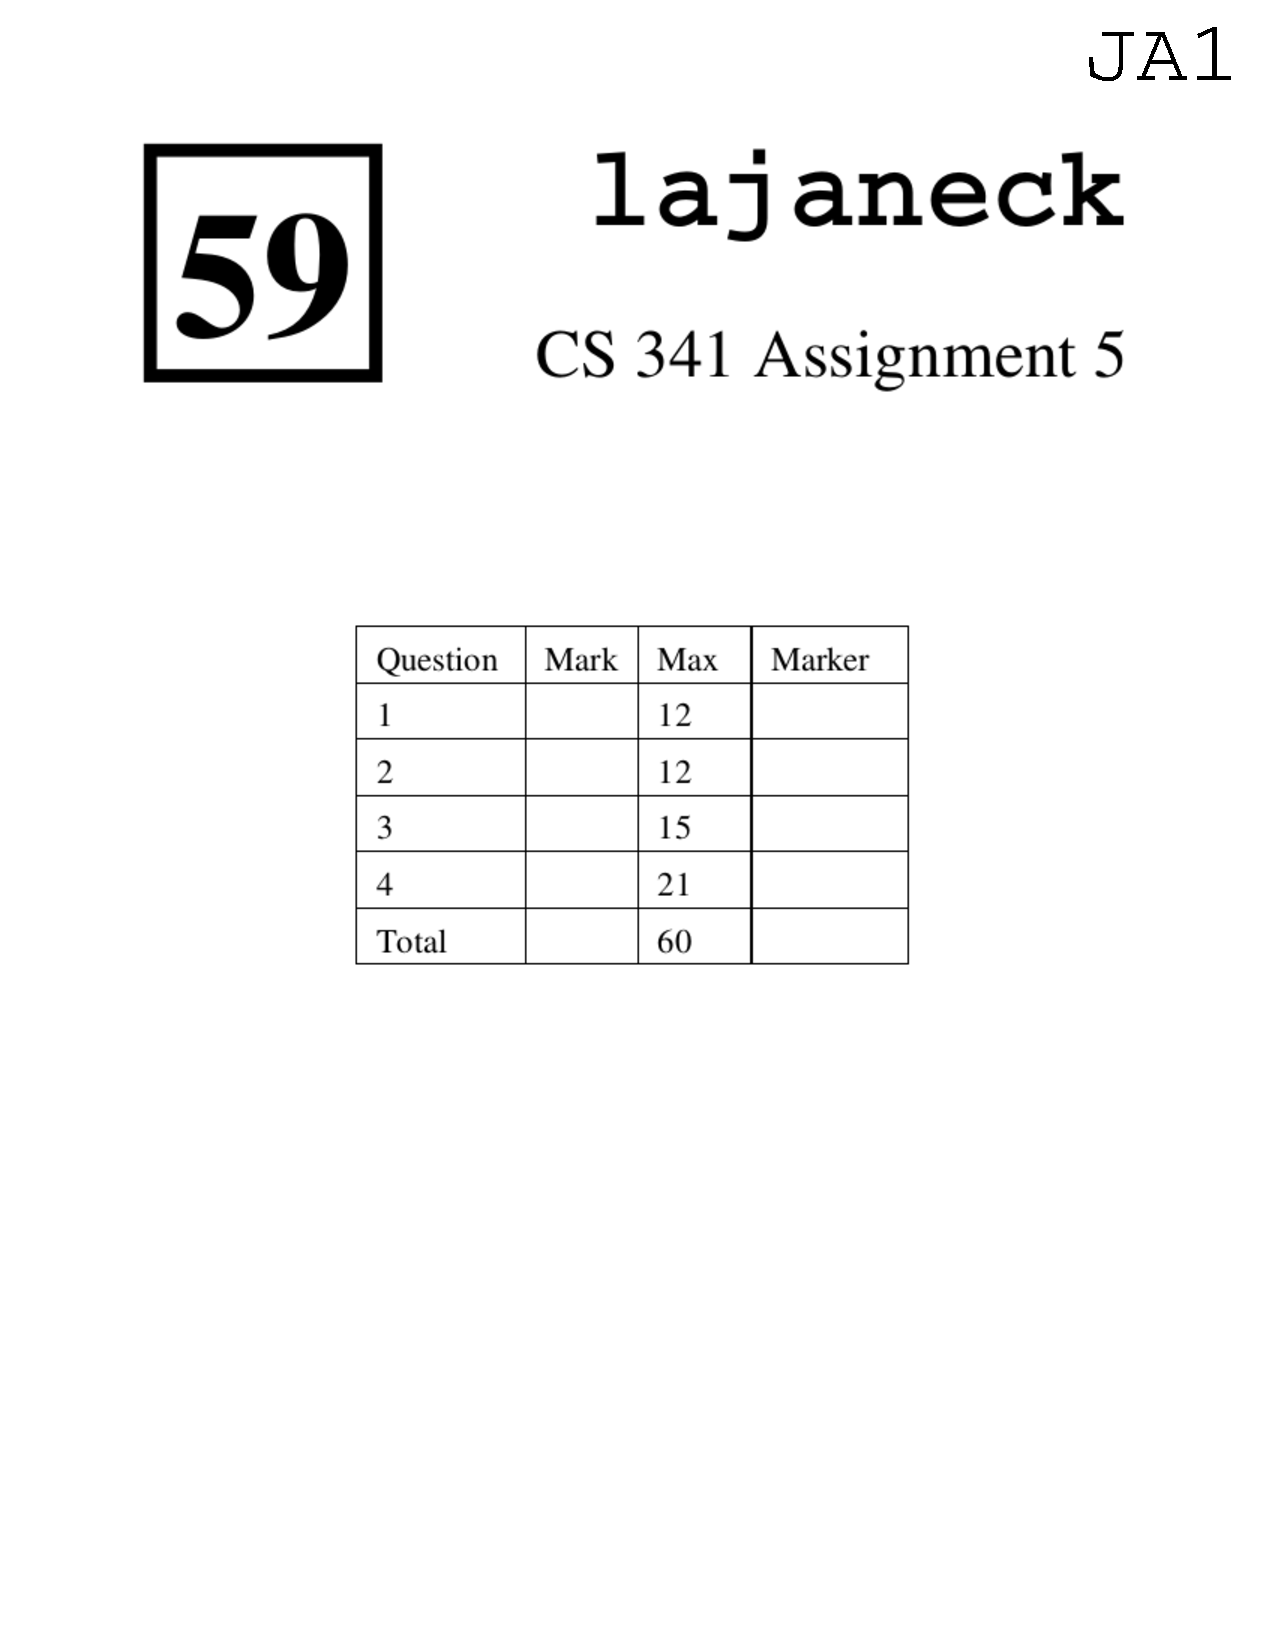
\includepdf[pages={1}]{cover.pdf}
\section*{Question 1}
\subsection*{a)}
Let every node on the graph be a tuple of two values, one representing the amount of water in the bigger jug (A) and one representing the amount of water in the smaller jug (B). Each edge of the graph represents the result of one of the following actions
\begin{itemize}
    \item filling jug A with water
    \item filling jug B with water
    \item emptying jug A
    \item emptying jug B
    \item pouring jug A into jug B
    \item pouring jug B into jug A
\end{itemize}
We build the graph by starting at (0,0), apply each of the possible actions (within the constraints of the jug sizes) and form new nodes where necessary. Continue this recursively for each new child node (if a child node already existed do not recurse on it).

Because we have bounds on how much water can be in each jug ($0 < A < n_1$ and $0 < B < n_2$) and each action works by adding integer amounts we have a bounded number of nodes. The three types of actions all result in integer values. Filling and emptying the jugs will result in 0, $n_1$, or $n_2$ values which are all known integers. Pouring jug B into jug A will always result in a multiple of $n_2$, or $n_1$ if the jug is filled. Similarly pouring jug A into jug B will result in one of the possible values for jug A or $n_2$ if the jug is filled. So each jug may only contain a multiple of $n_2$ (this includes 0) or $n_1$. Similarly, pouring jug A into jug B will result in jug A being size $n_1-n_2$, if we repeat this we will get $n_1$ minus a multiple of $n_2$. So jug A has $\mathcal{O}(\frac{n_1}{n_2})$ potential values, and jug B can be any of those values smaller than $n_2$ or $n_2$, so it is also bounded by $\mathcal{O}(\frac{n_1}{n_2})$. If we have a node for each possible combination of jug A and B sizes we will have $\mathcal{O}((\frac{n_1}{n_2})^2)$ possible nodes. Each node has at most 6 possible edges so our edge set is also bounded by $\mathcal{O}((\frac{n_1}{n_2})^2)$.

\subsection*{b)}
Either a BFS or DFS will work to solve this. Starting from ($n_1,n_2$) (although any node would work, this just makes it easier on John and Zeus who will want a good starting point) run either search algorithm and see if a node where the weight of jug A is $n_3$ is discovered.

The complexity of this is:
\begin{align*}
    \mathcal{O}(n+m) &= \mathcal{O}((\frac{n_1}{n_2})^2 + (\frac{n_1}{n_2})^2)\\
                     &= \mathcal{O}((\frac{n_1}{n_2})^2)\\
\end{align*}

\section*{Question 2}
\subsection*{a)}
The distance between the two sets is defined as the minumum distance between a point in one set and a point in the other. This will be the smallest weighted edge between the two sets since edges are weighted based on the distance between their points.

Using the lemma we know that the smallest weighted edge between the two sets will be in the MST. Which means that for any two subsets (that are disjoint and contain all points) their distance is the edge of the MST that connects them.

$P_1$ and $P_2$ are separated by removing e which means that the edge in the spanning tree that connected them was e (there can be no other edge because that would create a cycle in the MST), so the distance between $P_1$ and $P_2$ is the weight of the edge that was removed from the MST to separate them, so $w(e)$.

\subsection*{b)}
As stated above the distance between two sets of points will be the edge in the spanning tree between those two sets. Since e is the heaviest edge in the MST all other edges must be less than or equal to w(e). This means that the distance between any subsets is less than or equal to w(e). This also applies to the optimal solution.

If the distance of the optimal solution was greater than e there would have to be an edge in the MST with a heavier weight than e which is impossible since e was defined as the edge with the heaviest weight in the MST.

\subsection*{c)}
Our graph has a node for every point in g and Since we use our edges to define distance we cannot have two points without a connecting edge (there is no case where two points do not have a distance between them), so every node has degree n-1. Summing across every node we have $m \in \mathcal{O}(n^2)$

If we use Dijkstra's algorithm to make the MST with Fibonacci heaps we will have a run time of :
\begin{align*}
    \mathcal{O}(n\log n + m) &= \mathcal{O}(n\log n + n^2)\\
                            &=\mathcal{O}(n^2)
\end{align*}

In a) we proved that the distance between $P_1$ and $P_2$ is the weight of e and in b) we proved that the distance of the optimal solution is less than or equal to the weight of e. Since we are trying to maximize the distance between the two sets of our optimal solution we will chose the largest possible edge, e. If $P_1$ and $P_2$ were not the optimal solution, another edge in the spanning tree, would be the distance between $P_1^*$ and $P_2^*$. This edge would have to have weight higher than e because we are looking for the maximum and this solution must be more optimal than $P_1$ and $P_2$. The edge must also be less than or equal to e as proven in b). This is of course impossible, so there can be no solution more optimal than $P_1$ and $P_2$.


\section*{Question 3}
\subsection*{a)}
\textit{Input: }positive integers $v_1, \dots , v_n, w_1, \dots, w_n, W_1, W_2, V.$ \\
\textit{Output: } ``yes'' iff there exists disjoint subsets A, B $\in {1, . . . , n}$ such that $\sum_{k \in A}w_k \leq W_1$ and $\sum_{k \in B}w_k \leq W_2$ , where $\sum_{k \in A}v_k + \sum_{k \in B}v_k \geq V$.

This is still NP because the certificate is the two subsets A and B which are bounded by $\mathcal{O}(n)$ integers which have bit sizes $\mathcal{O}(\log U)$, so the size is $\mathcal{O}(n\log U)$ which is polynomial. To verify these we just need to calculate the sum of each subset and compare it to the given restrictions which can be done in $\mathcal{O}(n)$ time.

\subsection*{b)}
Since we cannot include the value of an item that does not exist the $\sum_{k \in A}v_k + \sum_{k \in B}v_k$ is bounded by $\sum_{i=0}^n v_i$. This means that any value of V higher than  $\sum_{i=0}^n v_i$ will never yield ``yes'' from the decision algorithm. We start by calling the decision algorithm on $V = \frac{1}{2} \sum_{i=0}^n v_i$ (at the center of possible values). If this returns ``yes'' we recurse on right half of values, if it returns ``no'' we recurse on the left half of values. We repeat this until a single value is reached, this is our maximum total.

This algorithm will call the decision matrix $\mathcal{O}(\log  \sum_{i=0}^n v_i)$ times which is still polynomial time.

\subsection*{c)}
Using a) we get the maximum total value. Then we iterate through the set of items removing items one at a time and checking if the maximum total has changed with this removal. If the maximum total has changed then that item is in the optimal solution and gets added back in, else we leave the item removed. Once we are done with this we will have the set of items that are in the optimal solution. This set is found by calling the subroutine to calculate the maximum value n times. Thus we have a polynomial times a polynomial which is still polynomial time.

Now that we have the set of items in the optimal solution we need to find which set they go in. To do this we iterate through each item (which is bounded by $\mathcal{O}(n)$ items) and pretend that the item is in set B by removing that item from the set of possible items and decreasing the allowed total weight of B by the weight of that item. With this reduced item set and set B weight we run the initial decision algorithm to see if there is still a solution. If it returns yes we leave the item in B else we put the item in A and keep going. This will result in n calls to the initial decision algorithm which its known to be polynomial time so this will also be done in polinomial time.

\section*{Question 4}
\subsection*{a)}
The certificate must contain less than n quadrilaterals (since it is impossible to have a subset larger than its parent set) each of which are made of 4 points; each point is a set of 2 integers. So our certificate is 8n integers which is bounded by $\mathcal{O}(n)$ integers which have bit sizes $\mathcal{O}(\log U)$, so the size is $\mathcal{O}(n\log U)$ which is polynomial.

To verify our answer we iterate through the k quadrilaterals and m points in the solution. For each point-quadrilateral pair we check if the point in is the quadrilateral. If ever there is a point that is in no quadrilateral we know that our solution is invalid. To do this we make km calls to the subroutine that checks if a point is in a quadrilateral. Since k is a constant this is bounded by $\mathcal{O}(m)$ calls to a polynomial function. Multiplying a polynomial function by a polynomial function results in a polynomial function so our verification can be done in polynomial time.

\subsection*{b)}
We know that Quad-Cover is a NP problem as proven in A. Now we need to find a polytime reduction from Vertex-Cover to Quad-Cover.

This is done by mapping each edge $(i,j)\in E, i<j$ to a point $(i,j)$ in P. We then map $a \in V$ to a rectangle $(0,a), (a, \texttt{MaxY}), (a,a), (a-1, a+1)$ in Q (maxY is the highest y value of the points).

Each quadrilateral is essentially an L shape containing all points that have the value ``a'' as its x or y coordinate, where a is the value of the associated vertex. We know that the quadrilateral will contain all points incident to its associated because it traces along the x values from (a,a) to 0 and along the y values from (a,a) to some max. We dont need to include the bottom triangle since the x and y values of the points are ordered no points will appear in the bottom triangle. So we only need this L shape to cover all incident points.

This is done in polytime since we are just mapping each edge and node using constant time operators.

\textbf{Proof of correctness: } There exists a vertex coverage of size k iff there exists a subset $T \subseteq Q$ of at most k quadrilaterals such that every point in P lies inside some quadrilateral in T, where P and Q are the sets defined above.

Proof($\Rightarrow$)
Suppose we have a k sized subset of Q, T that contains ever point in P.

Assume then that we do not have a vertex coverage of size k. This means that there is an edge ab in E that is not covered by the chosen vertexes V'. So vertexes a and b were not in V'. Since there is a one-to-one mapping between the vertex input and the quad input quadrilateral a and b were not in T. But when we map this edge to its point in P it has the coordinates (a,b). Each quadrilateral covers only points that have its value as either its x or y coordinate, so (a,b) can only be covered by quadrilateral a or b. But as stated above quadrilaterals a and b were both not chosen. This means that point (a,b) was not covered. This is a contradiction since we assumed that we have a quad coverage. Therefore having a vertex coverage of T of size k for quadrilateral Q and points P implies having a vertex coverage of a k sized subset of V (as mapped to Q) that covers all edges in E (as mapped to P).

Proof($\Leftarrow$)
Suppose we have a k sized subset of V, S, that covers every edge in E.

Assume that we do not have a k sized subset subset of Q, T, that contains every point in P. This means that there is a point (a,b) not covered by a quadrilateral. Since every quadrilatteral is designed to cover all points with its value in their x or y coordinate, the quadriallteras for a and b cannot be in T, else the point (a,b) would be covered. There is a one to one mapping between quadrilateral in Q and vertexes in S, so vertexes a and b cannot be S inf they are not in T. Since a and b are both not in S, the edge between a and b is not covered in the vertex covering of T. This is a contradiction since we assumed that we had a complete vertex coereing with T. Thus having a having a k sized vertex covering T implies having a k sized quad covering Q.

\subsection*{c)}
\begin{tabular}{|c|c||c|c|}
\hline
\textbf{E} & \textbf{P} & \textbf{N} & \textbf{Q}\\
\hline
12 & (1,2) & 1 & (0,1),(1,1),(1,7),(0.2)\\
\hline
23 & (2,3) & 2 & (0,2),(2,2),(2,7),(1.3)\\
\hline
34 & (3,4) & 3 & (0,3),(3,3),(3,7),(2.4)\\
\hline
25 & (2,5) & 4 & (0,4),(4,4),(4,7),(3.5)\\
\hline
26 & (2,6) & 5 & (0,5),(5,5),(5,7),(4.6)\\
\hline
36 & (3,6) & 6 & (0,6),(6,6),(6,7),(5.7)\\
\hline
46 & (4,6) & 7 & (0,7),(7,7),(7,7),(6.8)\\
\hline
47 & (4,7) & & \\
\hline
56 & (5,6) & & \\
\hline
67 & (6,7) & & \\
\hline
\end{tabular}

\textit{Note: To the poor individual that has to mark this, I appologize for my lackluster art skills.}

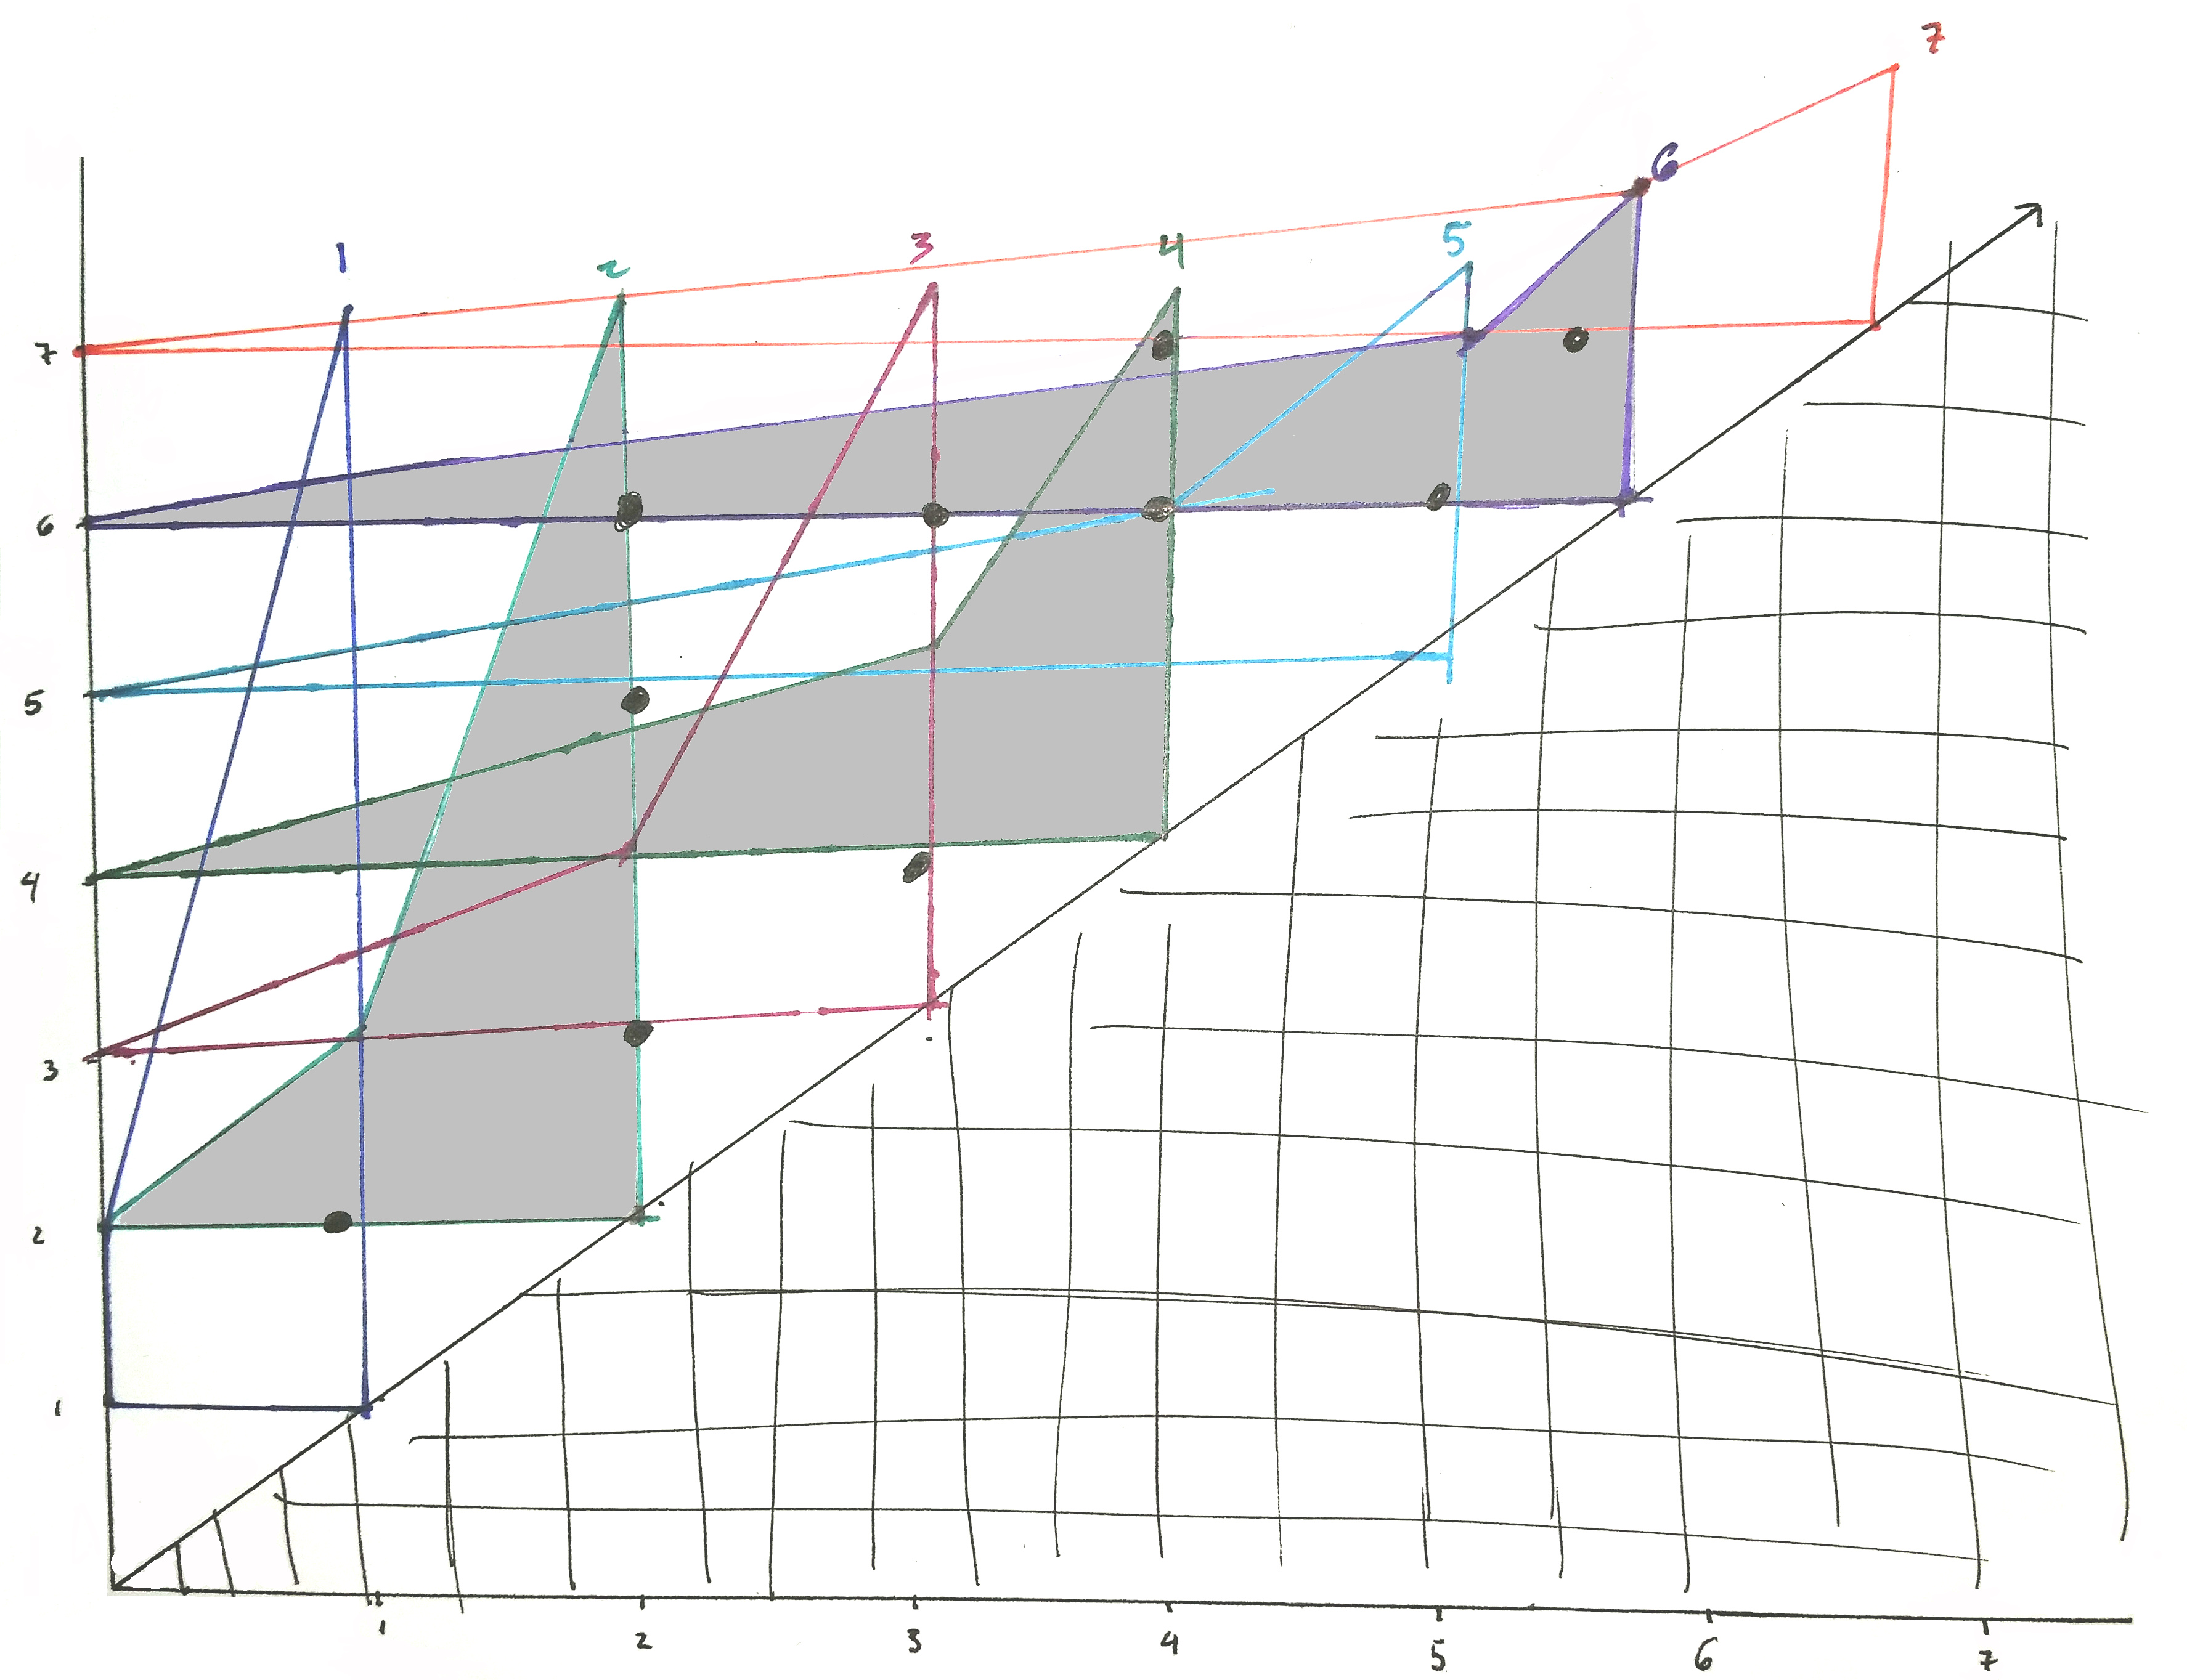
\includegraphics[scale=0.2, angle=90]{data}











\end{document}
